\chapter{Sprint 04 – Administration de la plateforme}
\section*{Introduction}

Le Sprint 04 est dédié à l’implémentation des fonctionnalités d’administration de la plateforme Swift Helpers. Ce module permet aux administrateurs de superviser les activités des utilisateurs (clients et prestataires), de valider les comptes, de suivre les ordres en temps réel et de gérer les services proposés.

L’objectif principal est de fournir à l’équipe de gestion un ensemble d’outils centralisés pour assurer le bon fonctionnement de la plateforme, en veillant à la qualité du service, à la fiabilité des données et à la fluidité des processus opérationnels.

Ce chapitre présente :
\begin{itemize}
  \item Le backlog fonctionnel de l’administration,
  \item Le diagramme de cas d’utilisation dédié à ce rôle,
  \item Les diagrammes de séquence et d’activité illustrant les processus métiers,
  \item Les interfaces Angular destinées à l’administrateur,
  \item Et un aperçu sur les implémentations backend et frontend associées.
\end{itemize}


\section*{Backlog du Sprint 04}
\begin{table}[H]
\centering
\begin{tabular}{|c|p{4.5cm}|c|p{5cm}|c|c|}
\hline
\textbf{ID US} & \textbf{User Story} & \textbf{ID Task} & \textbf{Tâche} & \textbf{Estimation} & \textbf{Responsable} \\
\hline

US04.01 & En tant qu’admin, je veux valider un compte prestataire. 
        & T04.01.1 & Bouton « Interview » + envoi du mail & 2h & Aziz \\
        \cline{3-6}
        & & T04.01.2 & Bouton « Onboard » + mise à jour DB & 2h & Aziz \\
\hline

US04.02 & En tant qu’admin, je veux gérer les services proposés.
        & T04.02.1 & Ajout / modification / suppression de services & 3h & Aziz \\
\hline

US04.03 & En tant qu’admin, je veux suivre les ordres en temps réel.
        & T04.03.1 & Connexion WebSocket et rafraîchissement dynamique & 4h & Aziz \\
\hline
\end{tabular}
\caption{Sprint Backlog – Administration de la plateforme}
\end{table}

\section*{Diagramme de cas d'utilisation}
\begin{figure}[H]
\centering
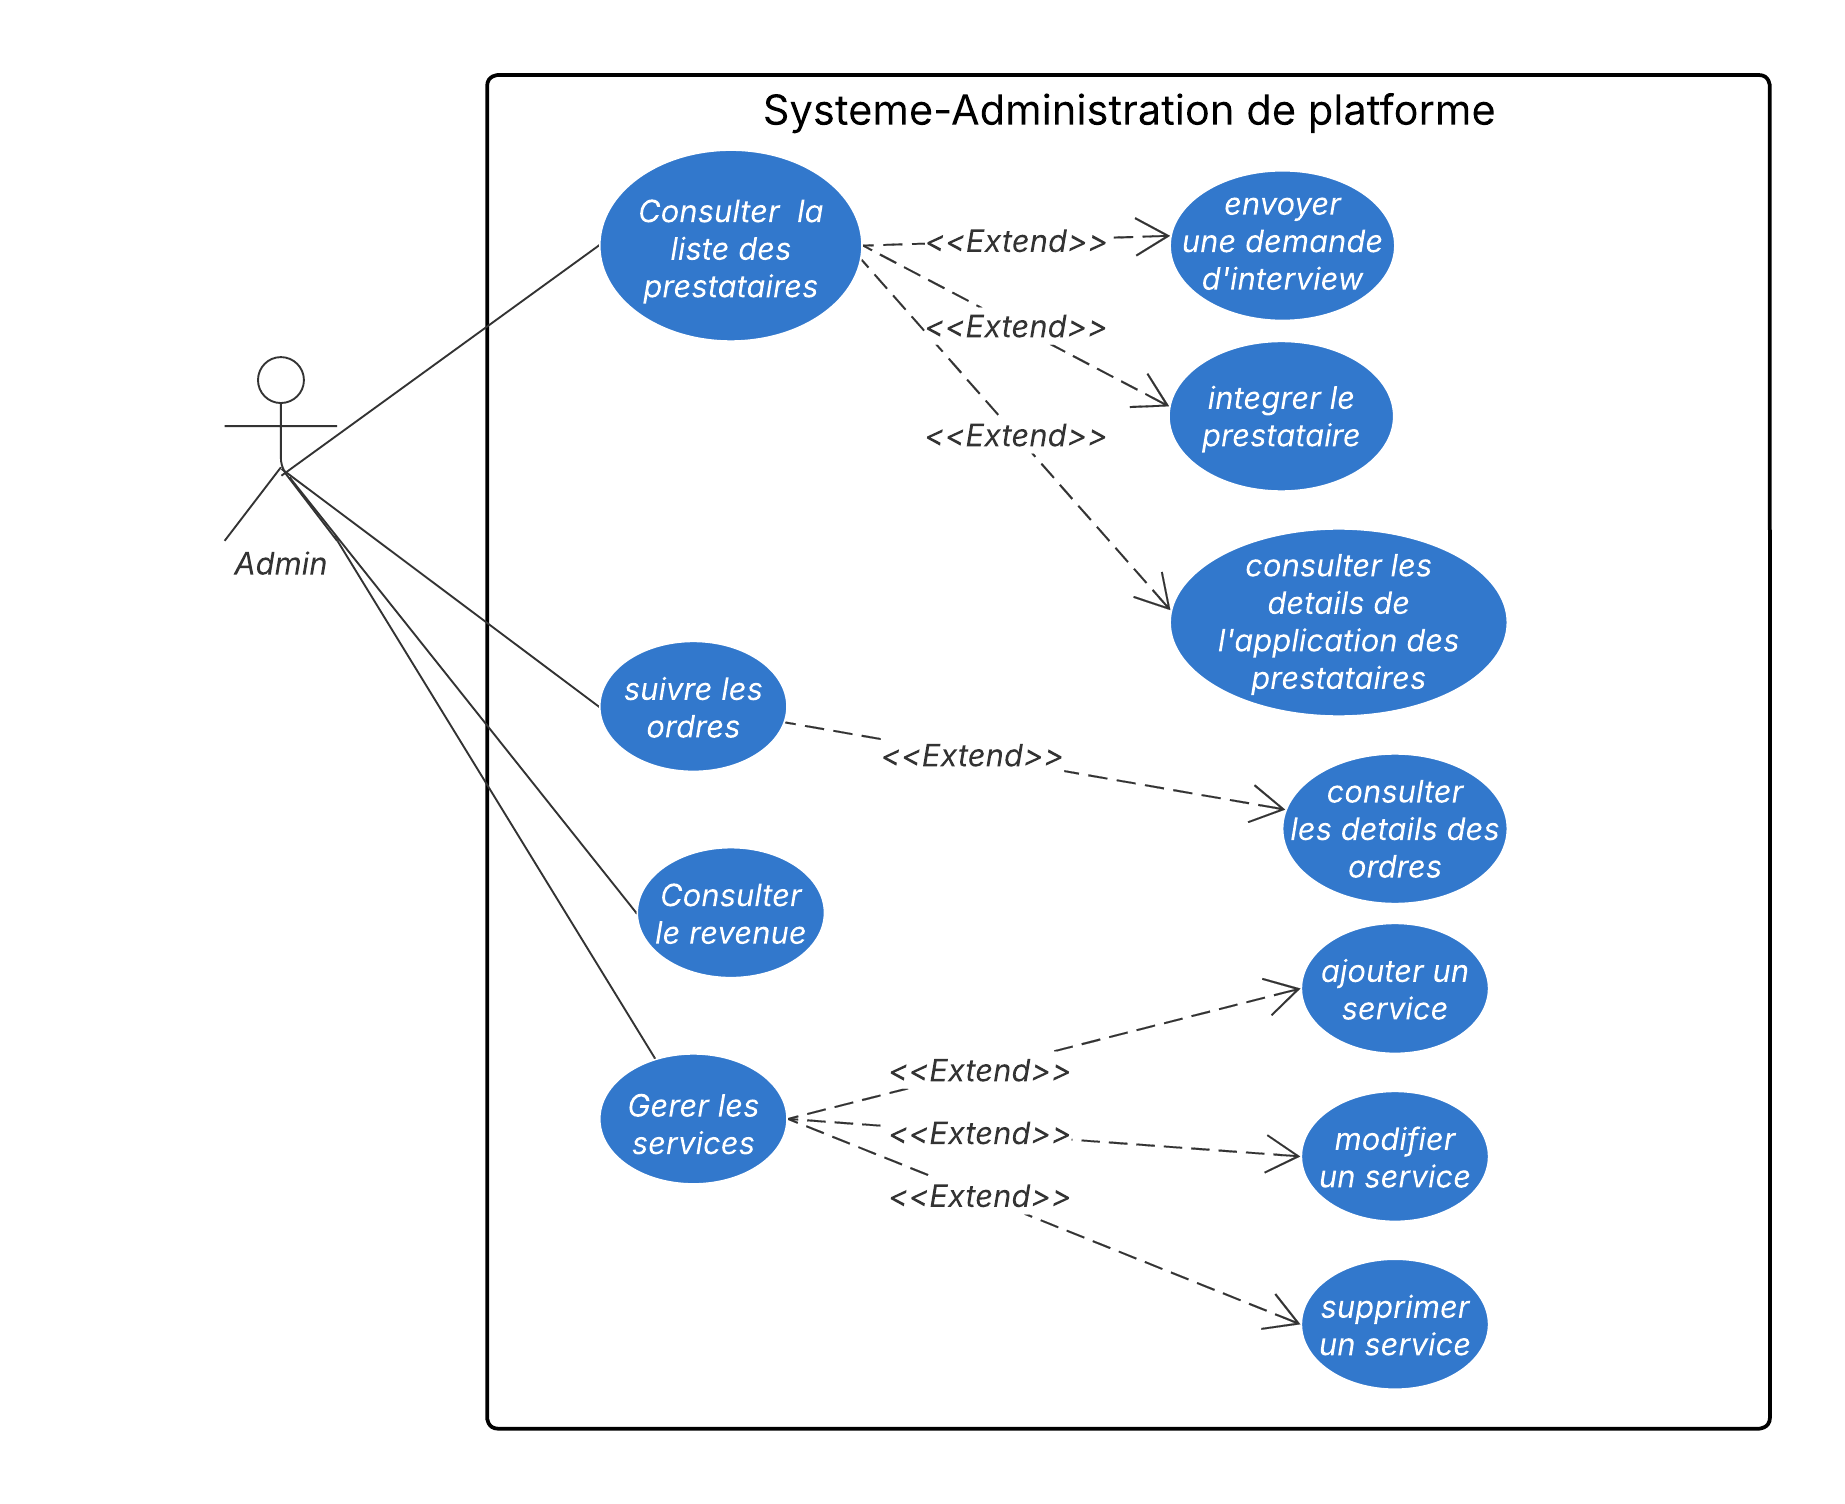
\includegraphics[width=0.85\linewidth]{figures/administration platforme.png}
\caption{Cas d'utilisation raffiné – Administration de la plateforme}
\end{figure}
\textit{Ce diagramme décrit les différentes actions que peut effectuer l’administrateur de la plateforme, notamment la validation des prestataires, la gestion des services, la supervision des ordres et la consultation des revenus.}

\section{Diagrammes de séquence}

\subsection*{Valider un compte prestataire (entretien + onboarding)}
\begin{figure}[H]
\centering
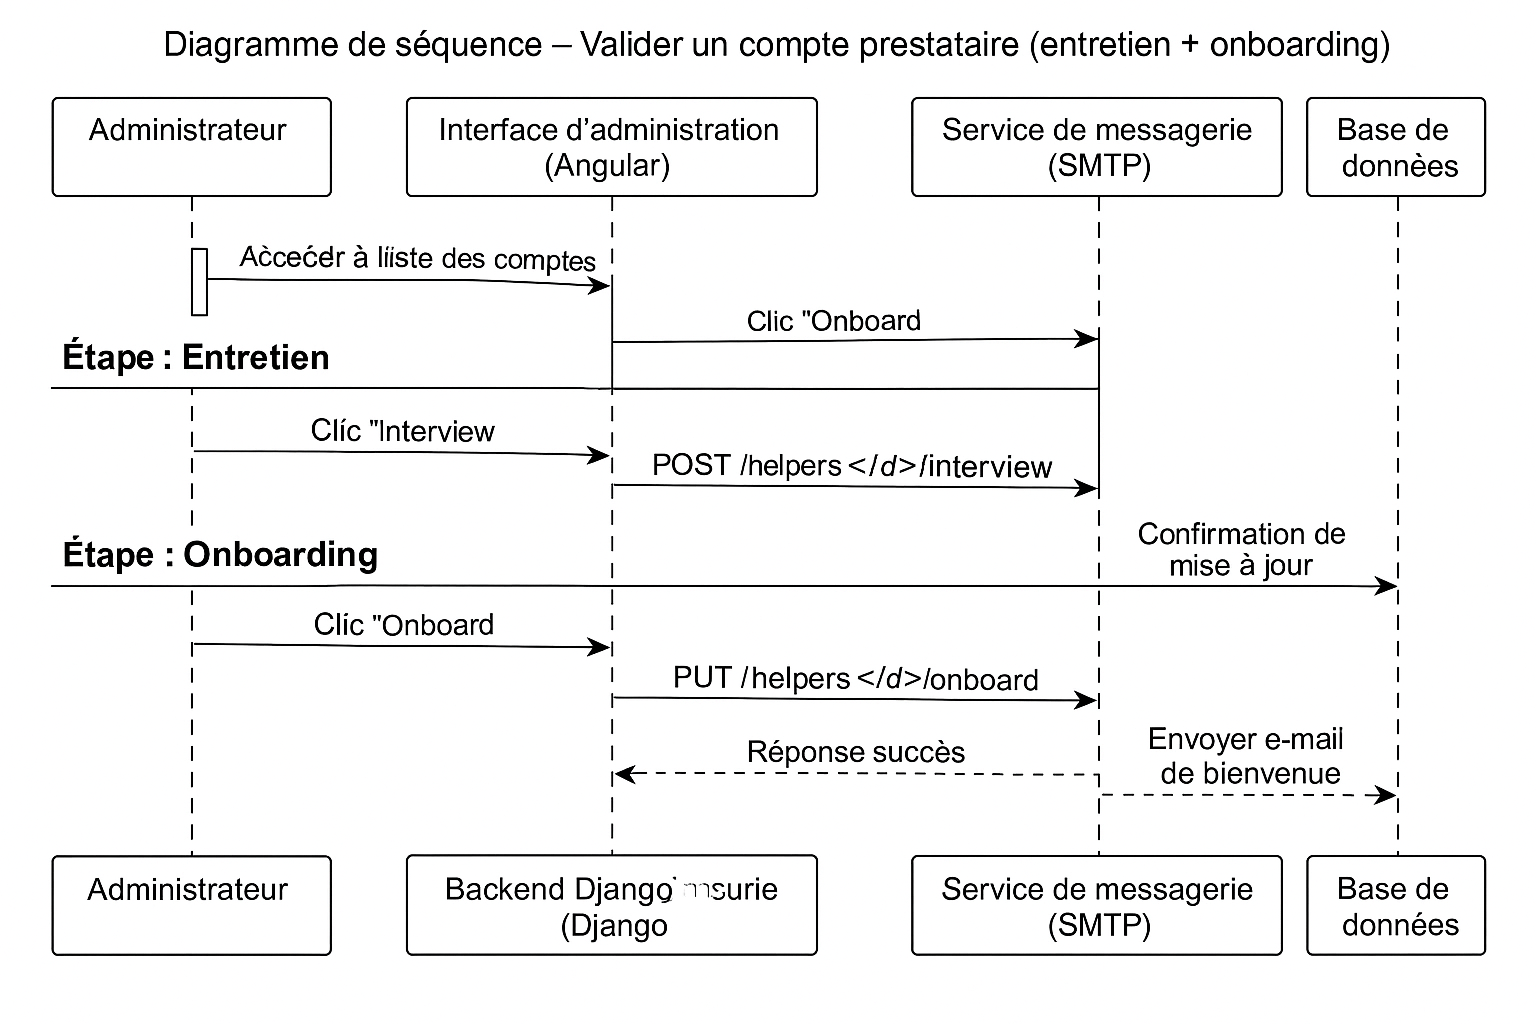
\includegraphics[width=0.90\linewidth]{figures/validation compte seq.png}
\caption{Séquence de validation d’un compte prestataire}
\end{figure}
\textit{Ce diagramme décrit les deux étapes successives : l’entretien (« Interview ») et l’activation (« Onboard ») du compte prestataire.}

\subsection*{Gérer les catégories de services}
\begin{figure}[H]
\centering
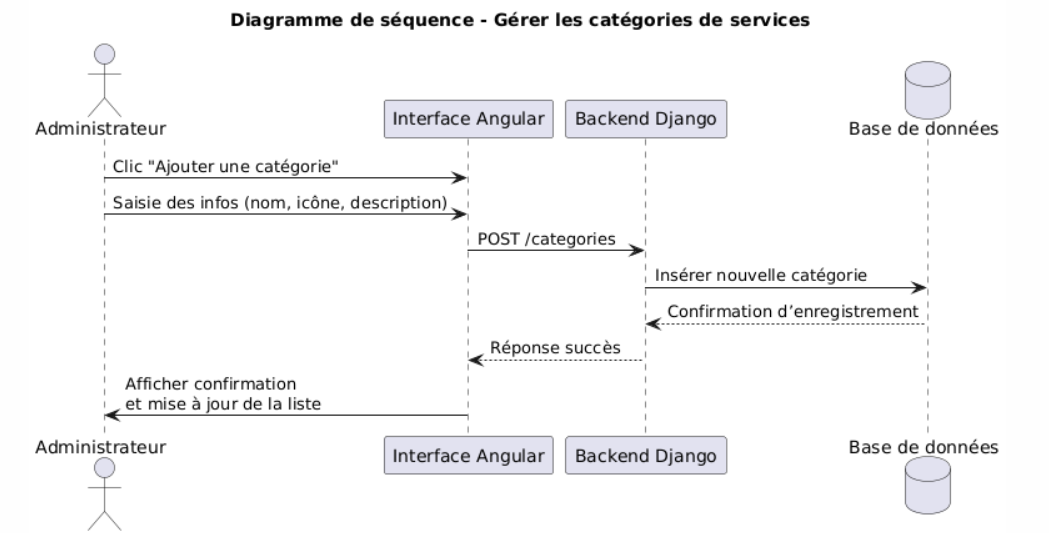
\includegraphics[width=0.85\linewidth]{figures/gestion des service seq.png}
\caption{Séquence – Gestion des catégories de services}
\end{figure}
\textit{L'administrateur ajoute, modifie ou supprime une catégorie de service. Le backend traite la requête et confirme la mise à jour.}

\subsection*{Suivi en temps réel des ordres}
\begin{figure}[H]
\centering
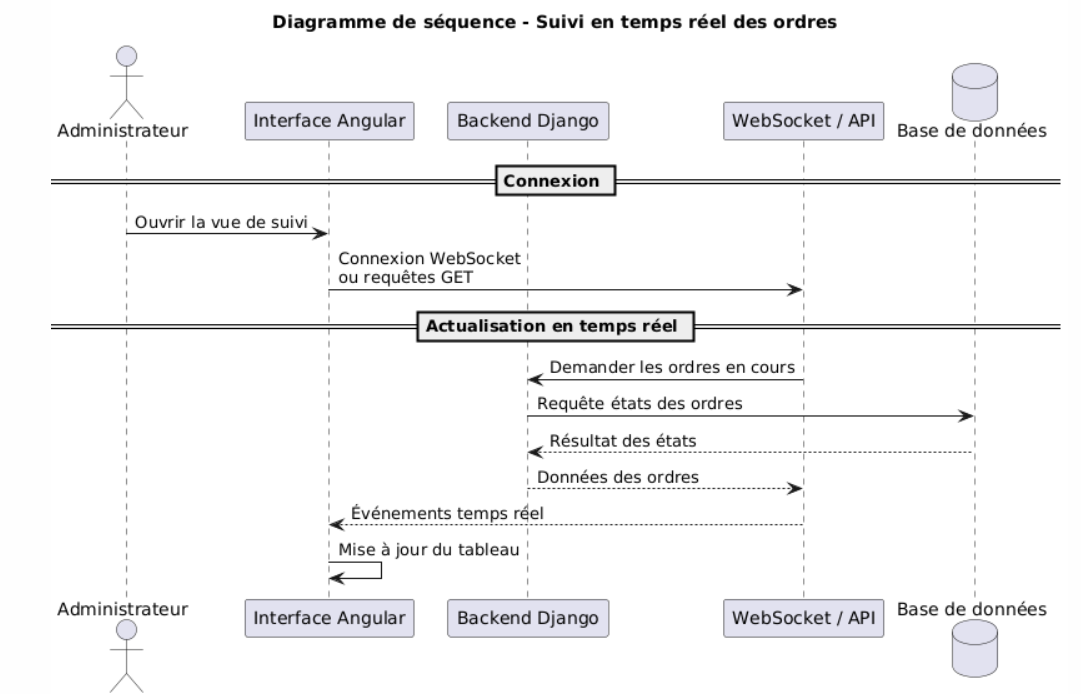
\includegraphics[width=0.85\linewidth]{figures/suivi des ordres seqq.png}
\caption{Séquence – Suivi en temps réel des ordres}
\end{figure}
\textit{La vue admin établit une connexion (WebSocket ou polling) pour afficher les mises à jour dynamiques des états des ordres.}

\section{Diagrammes d’activité}

\subsection*{Processus de validation d’un prestataire}
\begin{figure}[H]
\centering
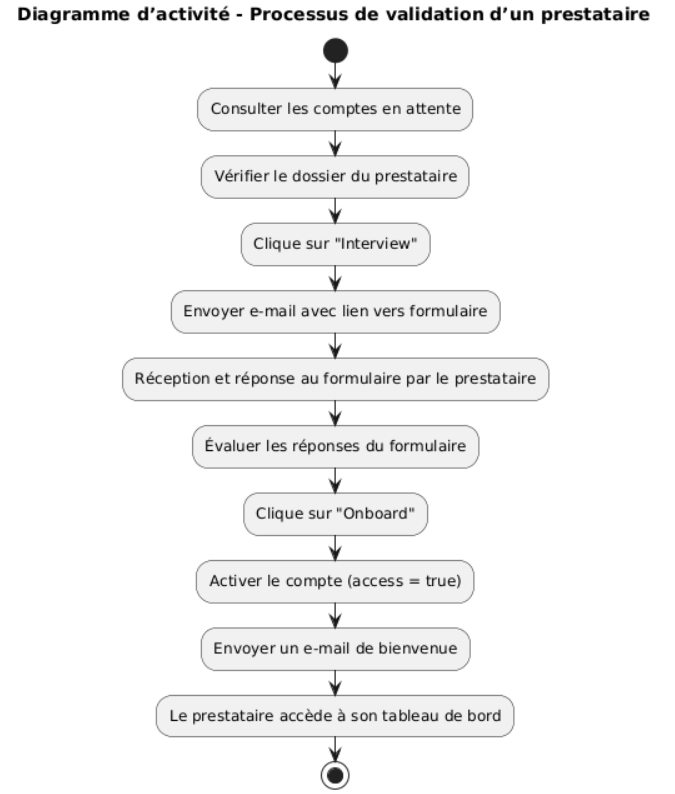
\includegraphics[width=0.75\linewidth]{figures/validation prestataire act.png}
\caption{Activité – Validation d’un compte prestataire}
\end{figure}
\textit{Ce diagramme montre les étapes de vérification du dossier jusqu’à l’activation du compte prestataire.}

\subsection*{Gestion des catégories de services}
\begin{figure}[H]
\centering
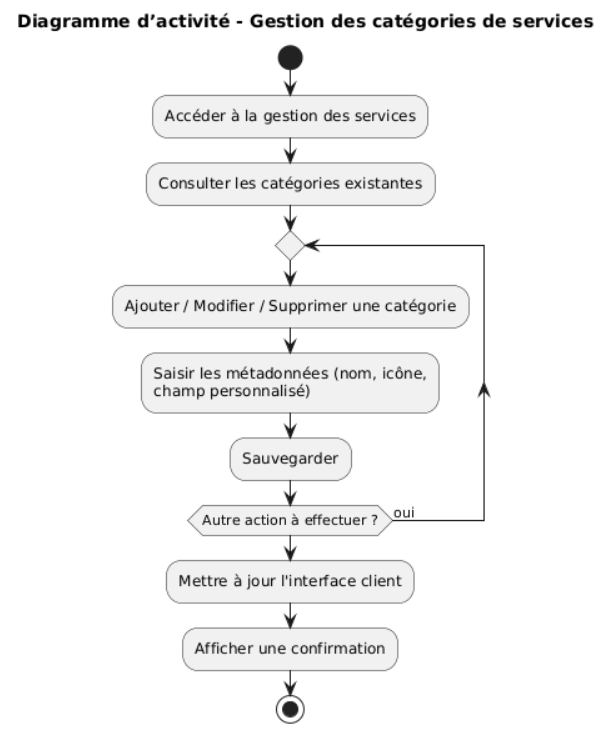
\includegraphics[width=0.75\linewidth]{figures/gestion des service act.png}
\caption{Activité – Gestion des services}
\end{figure}
\textit{L'administrateur peut parcourir les services existants, créer ou modifier une catégorie, et sauvegarder les données.}

\subsection*{Supervision des ordres de mission}
\begin{figure}[H]
\centering
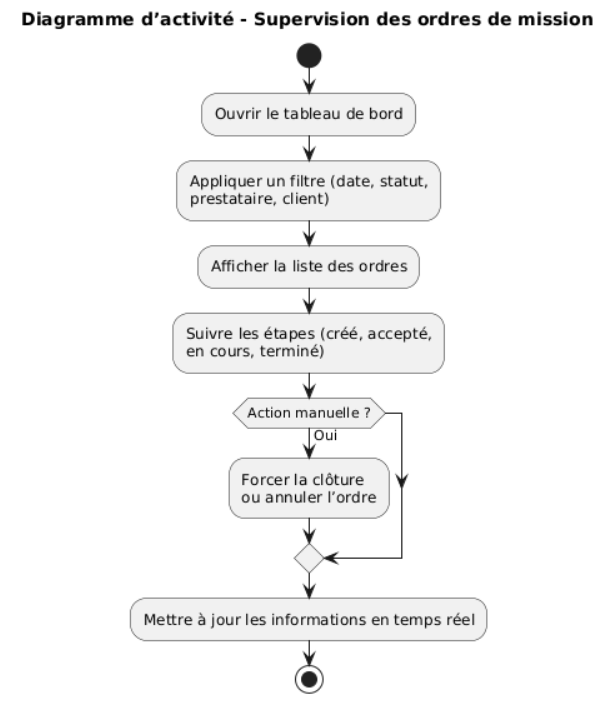
\includegraphics[width=0.75\linewidth]{figures/supervision des ordres act.png}
\caption{Activité – Supervision des ordres}
\end{figure}
\textit{Permet à l’admin de filtrer et d’intervenir manuellement sur les ordres en cours.}

\section*{Interface utilisateur – Angular}

\begin{figure}[H]
\centering
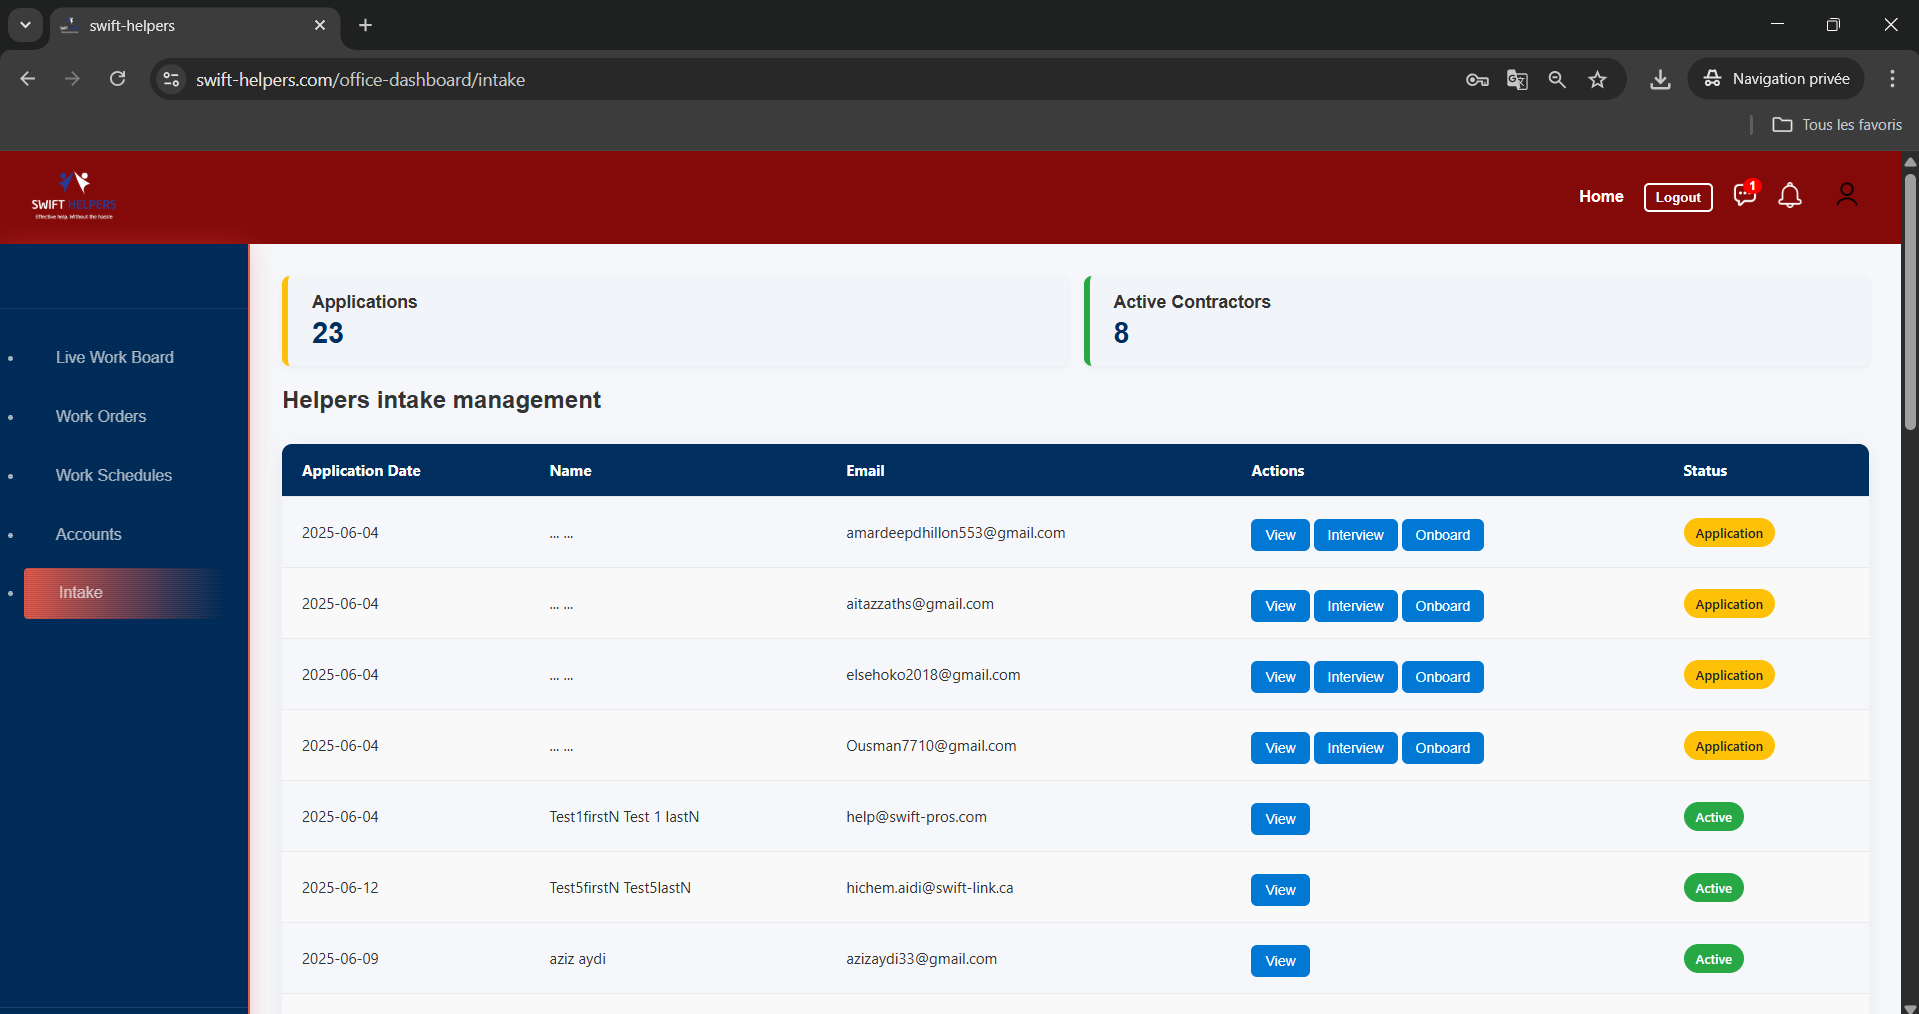
\includegraphics[width=0.85\linewidth]{figures/suivi prestataire.png}
\caption{Interface de gestion des comptes prestataires}
\end{figure}
\textit{Cette interface permet à l’administrateur de visualiser les candidatures reçues, de lancer les entretiens via le bouton \textbf{Interview}, puis de valider un prestataire via \textbf{Onboard}.}

\begin{figure}[H]
\centering
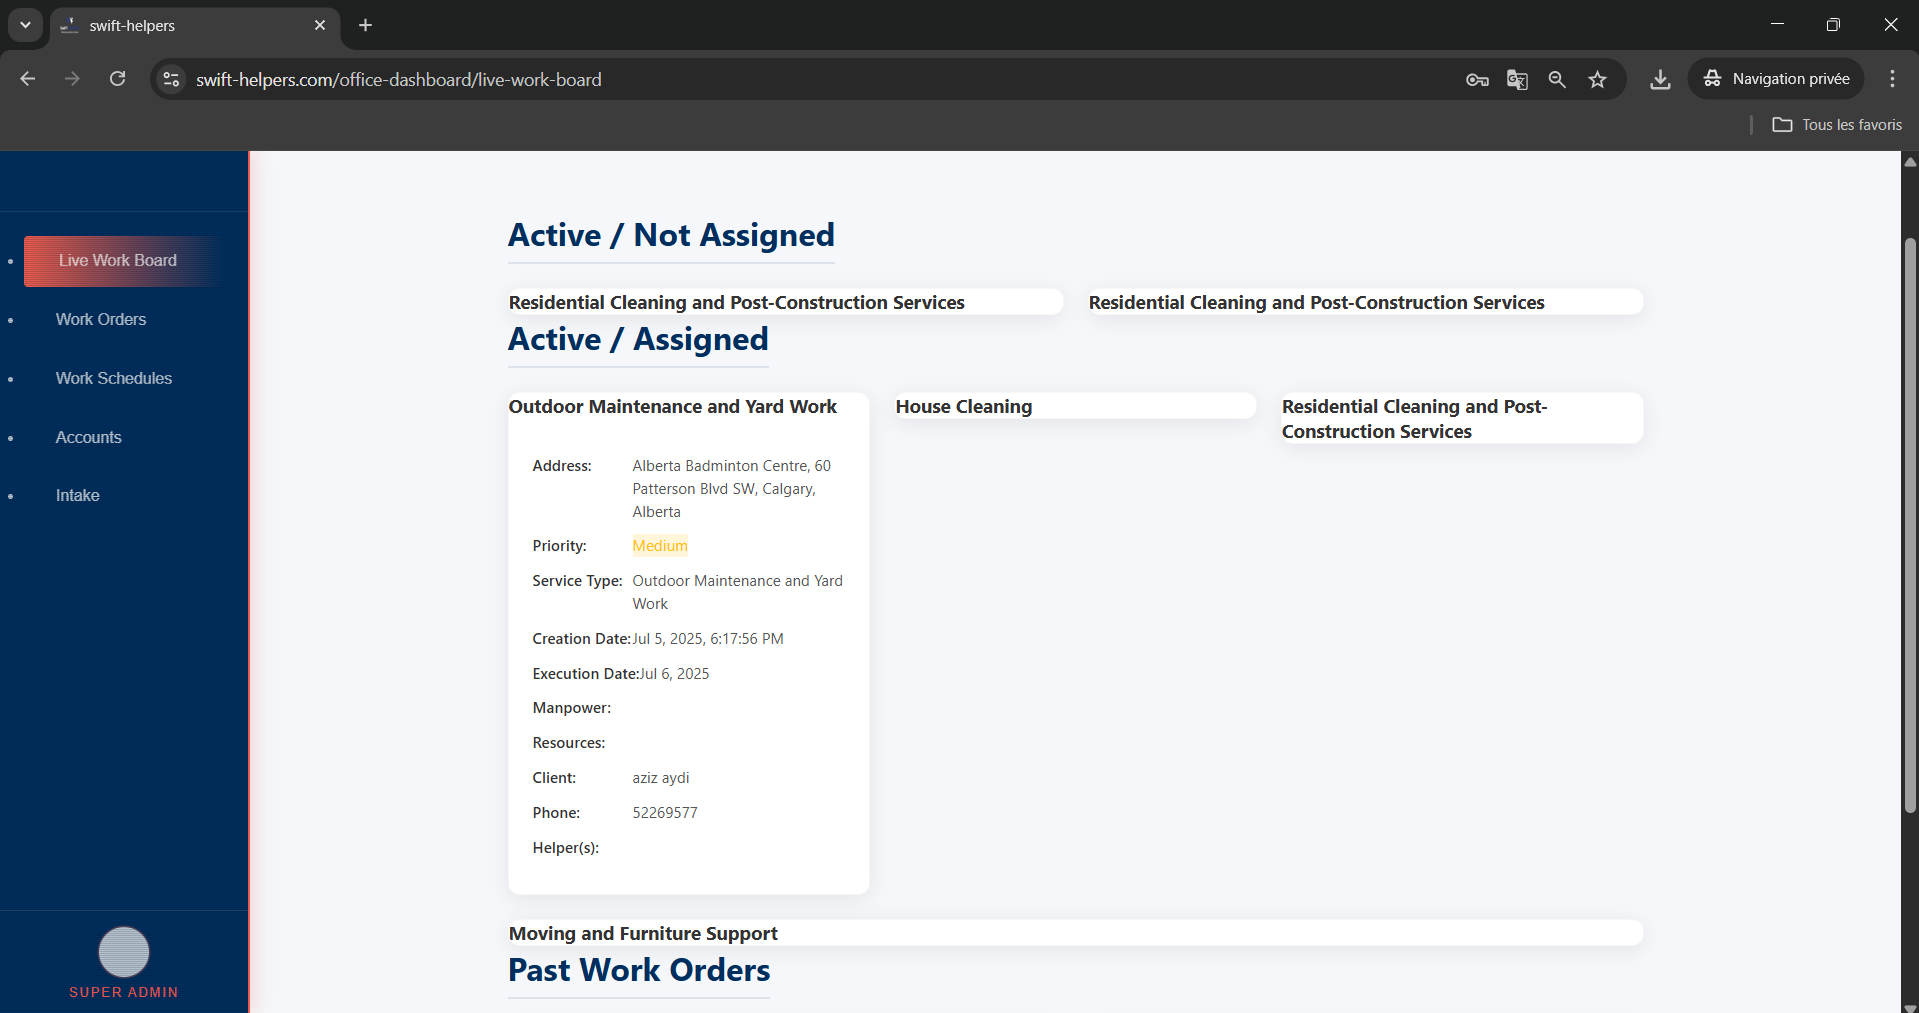
\includegraphics[width=0.85\linewidth]{figures/suivi orders.png}
\caption{Suivi en temps réel des ordres de mission}
\end{figure}
\textit{L’interface affiche dynamiquement les ordres actifs, assignés ou non, avec détails complets : priorité, client, date d’exécution. Elle est mise à jour automatiquement grâce aux WebSockets.}

\begin{figure}[H]
\centering
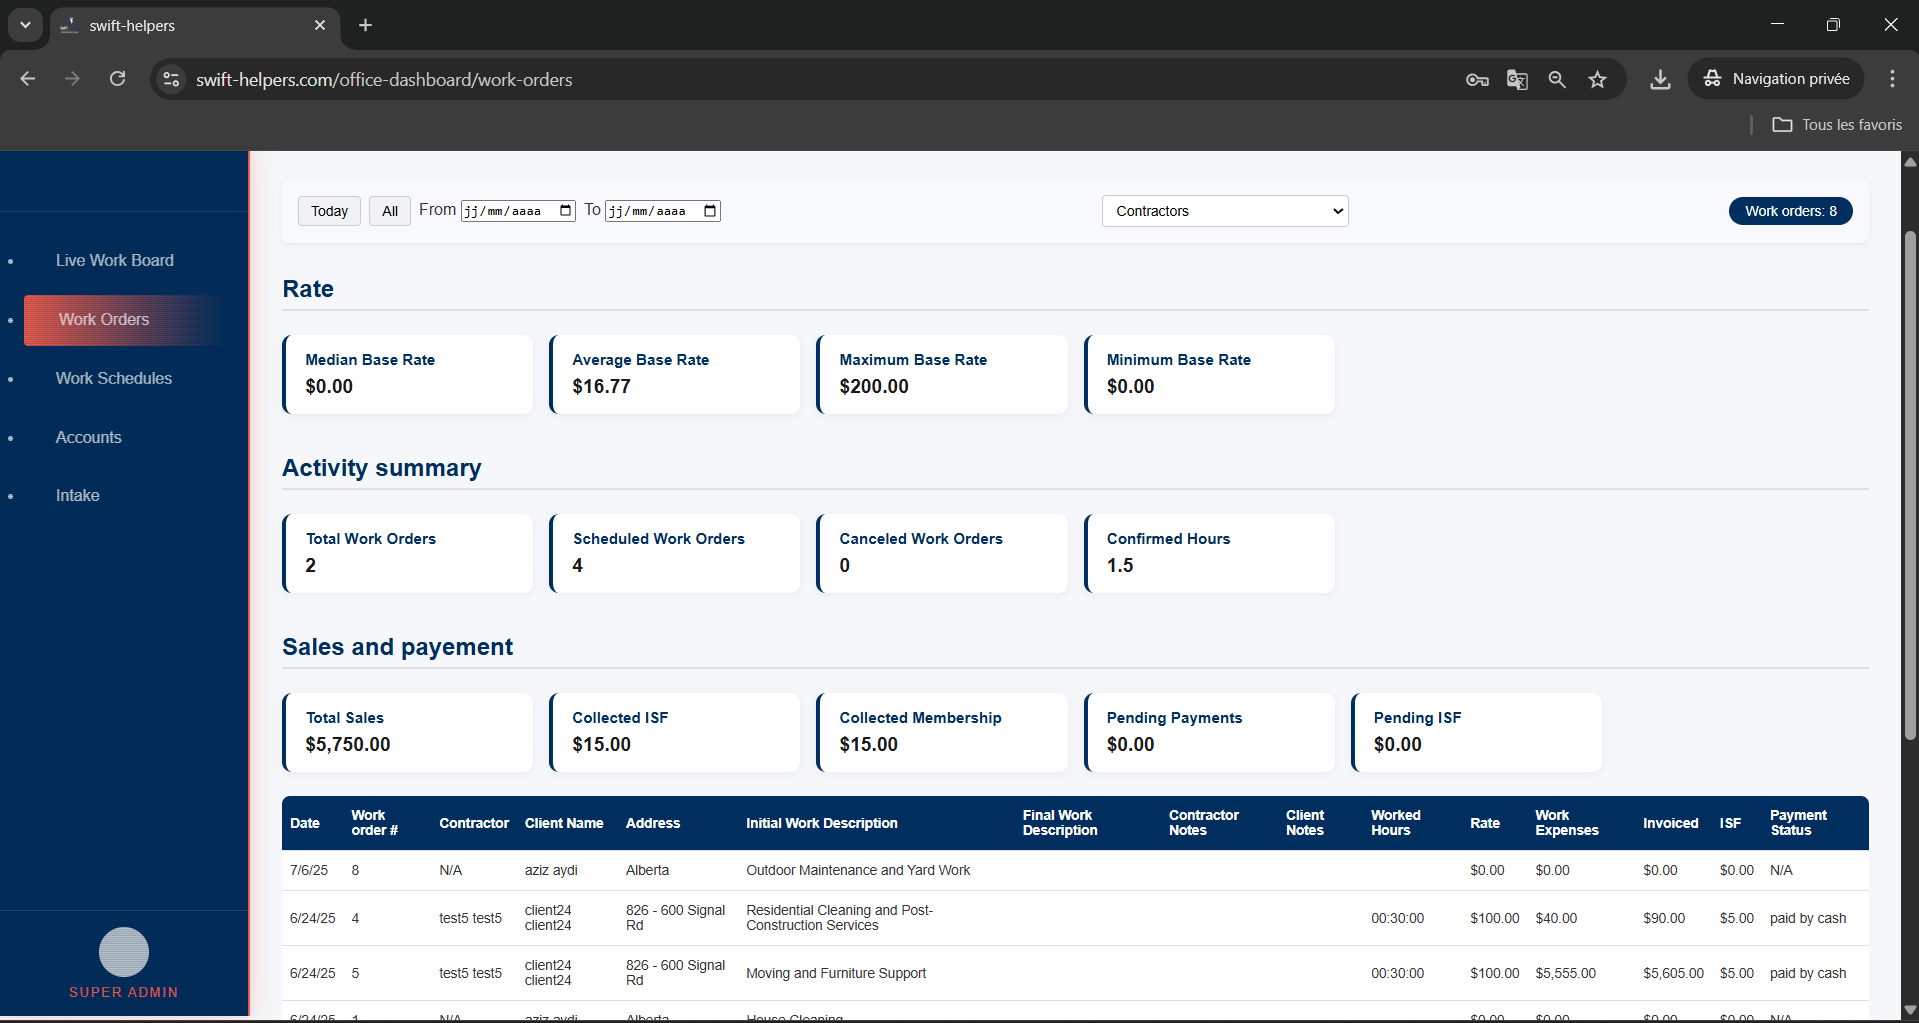
\includegraphics[width=0.85\linewidth]{figures/suivi revenue.png}
\caption{Suivi des revenus et des ordres}
\end{figure}
\textit{L’interface admin fournit des statistiques globales sur les revenus, les heures travaillées, et les ordres générés, avec possibilités de filtrage par période.}
\section*{Aperçu sur le code}

\subsection*{Frontend (Angular)}
\begin{figure}[H]
\centering
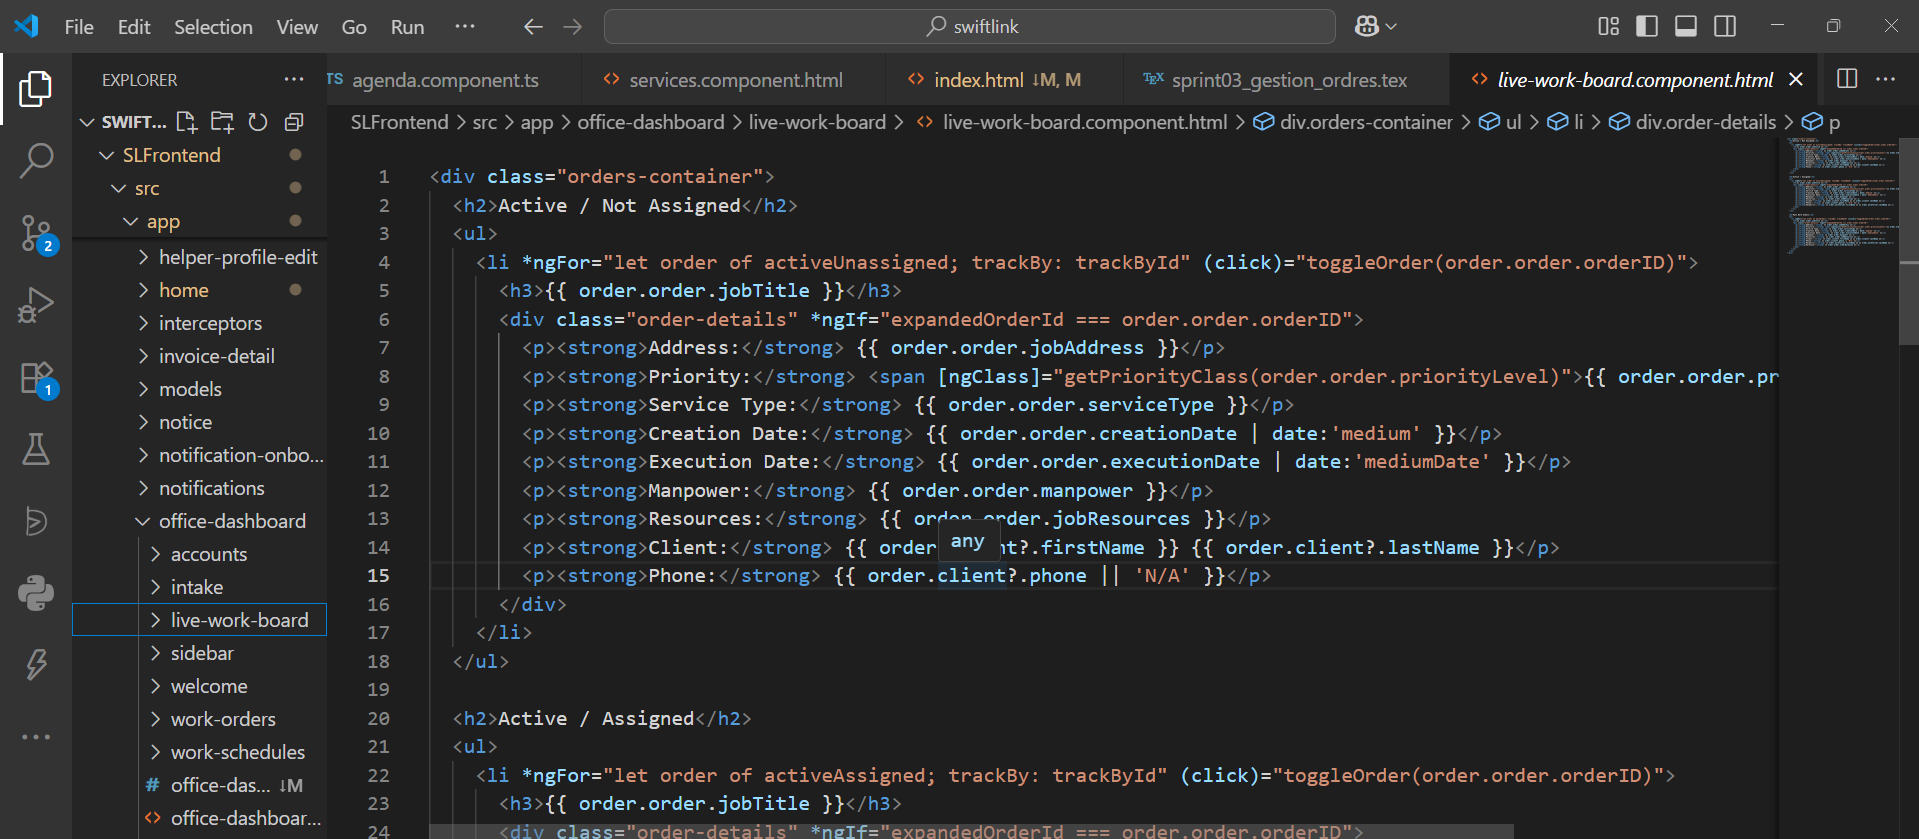
\includegraphics[width=0.85\linewidth]{figures/aperc front.png}
\caption*{\textit{Composant Angular affichant dynamiquement les ordres actifs et assignés, avec détails structurés, en vue admin.}}
\end{figure}
\textit{Les données sont affichées par boucle \texttt{*ngFor}, les classes CSS sont conditionnelles pour la priorité. Les ordres sont récupérés en temps réel via WebSocket ou polling périodique.}

\section*{Conclusion}

Ce sprint a permis de doter la plateforme d’un véritable tableau de bord d’administration, indispensable à la gestion et à la supervision du système en production. Les fonctionnalités développées – validation des prestataires, gestion des services, suivi en temps réel des ordres – renforcent le contrôle et la réactivité de l’équipe gestionnaire.

L’intégration d’outils comme la messagerie interne, la visualisation des revenus ou encore l’interface de suivi des missions permet d’assurer une gouvernance efficace de la plateforme, en s’appuyant sur des outils techniques fiables et ergonomiques.

Cette étape clôture le développement fonctionnel de la plateforme en fournissant aux administrateurs les leviers nécessaires à son exploitation quotidienne, tout en garantissant l’évolutivité future du système.



